\documentclass[12pt]{article}

\usepackage{CSPArticleStyle}

% - - - - - - - - - - - - - - - - - - - - - - - -
% additional packages
% - - - - - - - - - - - - - - - - - - - - - - - -
\usepackage{csquotes}
\usepackage[margin=1in]{geometry}
\usepackage{xypic}
\usepackage{booktabs}
\usepackage{parskip}
\usepackage{amsmath}
\usepackage{amsthm}
\usepackage{subcaption}
% Font settings - Times New Roman
\usepackage{times}
\usepackage[T1]{fontenc}
\usepackage[utf8]{inputenc}
\usepackage{CJKutf8}
\usepackage{float}

\bibliography{references.bib}


\title{From Controversy to Consensus: Modeling Community-Sensitive Common-Ground Management in German Discourse Markers}
\author{Hening Wang, Yuhan Guo, TBD}
\date{}

\begin{document}
%\maketitle

\textbf{\large From Controversy to Consensus: Modeling Community-Sensitive Common-Ground Management in German Discourse Markers}

Considering the sentences in (\ref{ex:intro}):

\begin{exe}
\ex \label{ex:intro}
Professor Weber kündigt (sofern ich weiß / wie du ja weißt / wie wir wissen / ja / bekanntlich) nächste Woche, deshalb sollten wir eine Abschiedfeier planen.\\
Professor Weber resigns as.far.as I know / as you \textsc{prt} know / as we know / \textsc{prt} / well.known next week therefore should we a farewell.party plan\\
`Professor Weber is resigning next week (as far as I know / as you know / as we know / you know / as is well known); therefore we should plan a farewell party.'
\end{exe}

These markers in parentheses systematically affect both the interpretation of $p$ and the consequent $q$. First, they form a hierarchy reflecting the degree to which the antecedent proposition $p$ is presented as shared within the relevant epistemic community, ranging from weak epistemic limitation (\textit{sofern ich weiß}) to strong public accessibility (\textit{bekanntlich}). Second, sharedness is context-dependent in two ways. It depends both on properties of $p$ (e.g., whehter Professor Weber is publicly known) and on how the relevant epistemic community construed (e.g., colleagues vs. the general public). Marker felicity therefore hinges on assumptions about how $p$ is evaluated as shared within a contextually determined epistemic community. Third, these markers also show a gradient hierarchy of speaker commitment to $q$, thereby increasing persuasive force. In this sense, marker choice reflects not only assumptions about shared knowledge, but also the speaker's own belief strength and argumentative goal.

This study focuses on a class of German discourse markers --- \textit{ja}, \textit{wie wir wissen} (`as we know'), and \textit{bekanntlich} (`as is well known') --- which we group under the label \emph{consensus markers}. Previous accounts have largely concentrated on the particle \textit{ja}. It is commonly assumed not to contribute to the truth-conditional content of $p$ \citep{gutzmann2015use,grosz2021discourse}, but to add expressive meaning that functions as a reminder, reactivating information already in the common ground salient. Accordingly, \textit{ja} has been described as marking $p$ as \textsc{known} \citep{thurmair1989modalpartikeln}, as indicating (speaker-assumed) common knowledge \citep{karagjosova2004meaning}, or as conveying that $p$ is uncontroversial \citep{jacobs_semantics_1991,zimmermann2011discourse,waltereit2001modal}. While these formulations converge on the intuition that $p$ is treated as settled, they are typically categorical rather than gradient and do not provide a basis for quantitative predictions. At the same time, it has been observed that \textit{ja} can be used as a common-ground management tool to strategically support broader communicative goals \citep{repp2013common}, the so-called ``manipulative use'' \citep{doring2016modal}. By presenting $p$ as uncontroversial, the speaker may facilitate discourse continuation and promote stability in the evolving discourse structure. Recent experimental work \citep{seemann2025} further suggests that the use of \textit{ja} is closely tied to causal reasoning contexts, where $p$ functions as a premise for subsequent argumentative moves.

Building on these insights, we argue that two aspects have not yet been sufficiently integrated into a unified formal account. First, notions such as sharedness and controversy are gradient rather than categorical: a proposition may be more or less widely shared and more or less controversial depending on community-specific background assumptions or world knowledge. Second, consensus marker use involves theory-of-mind reasoning: speakers must estimate interlocutors' epistemic states, the distribution of beliefs in the relevant community, and their own degree of commitment to an argumentative goal (e.g.\ convincing others to accept $q$ on the basis of $p$ as in example \ref{ex:intro}). We therefore propose a framework within probabilistic pragmatics \citep{goodman2016pragmatic,degen2023rational,franke2016probabilistic} that models consensus markers as encoding soft threshold constraints over a utility function integrating graded common-ground alignment, community-relative perceived controversy, and goal-directed speaker commitment, yielding explicit and testable predictions about marker choice across contexts.

\textbf{Formal model.}
We model a pragmatic listener as reasoning over latent perceived controversy $pc$ and speaker goal strength $g$ upon observing a consensus marker $u$. Perceived controversy decomposes multiplicatively as $pc = pc_{\mathrm{prop}} \cdot pc_{\mathrm{prag}}$, where $pc_{\mathrm{prop}} \in [0,1]$ captures propositional controversy and $pc_{\mathrm{prag}} \in [0,1]$ captures pragmatic controversy within the relevant epistemic community; $g \in [0,1]$ encodes the speaker's commitment to advancing the consequent $q$. Marker felicity is defined over a utility function
\[
U(pc,g) = w_g \cdot g - w_{pc}\cdot pc - w_{\mathrm{int}}\cdot(pc\cdot g),
\]
where the interaction term penalises persuasive effort under controversy. Each marker $u_i$ licenses the interval $[\theta_i, \theta_{i+1})$; thresholds are noisy latent variables $\theta_i \sim \mathcal{N}(\mu_i, \sigma_i^2)$, capturing graded overlap between adjacent markers. Marginalising over threshold uncertainty gives the interval likelihood
\[
P(u_i \mid pc, g)
\;\propto\;
\mathbb{E}_{\theta_i}\!\left[\sigma\!\bigl(\lambda\,(U - \theta_i)\bigr)\right]
\cdot
\mathbb{E}_{\theta_{i+1}}\!\left[\sigma\!\bigl(-\lambda\,(U - \theta_{i+1})\bigr)\right],
\]
which admits a closed form via the probit approximation; larger $\sigma_i$ softens the boundary, $\sigma_i \to 0$ recovers a hard threshold. The ordered mean thresholds $\mu_{\textit{sofern}} < \cdots < \mu_{\textit{bekanntlich}}$ ensure that stronger markers shift the posterior toward lower $pc$ and higher $g$. The listener recovers latent states by Bayesian inversion,
\[
P(pc_{\mathrm{prop}}, pc_{\mathrm{prag}}, g \mid u_i)
\;\propto\;
P(u_i \mid pc, g)\,P(pc_{\mathrm{prop}})\,P(pc_{\mathrm{prag}})\,P(g),
\]
and action adoption is a downstream logistic decision over the joint posterior:
\[
P(\mathrm{Adopt}(q) \mid u)
= \iiint
\sigma(\eta_0 + \eta_g g - \eta_{pc}\, pc - \eta_{\mathrm{int}}\, g \cdot pc)
\; P(pc_{\mathrm{prop}}, pc_{\mathrm{prag}}, g \mid u)
\; dpc_{\mathrm{prop}}\, dpc_{\mathrm{prag}}\, dg,
\]

\begin{figure}[h!]
  \centering
  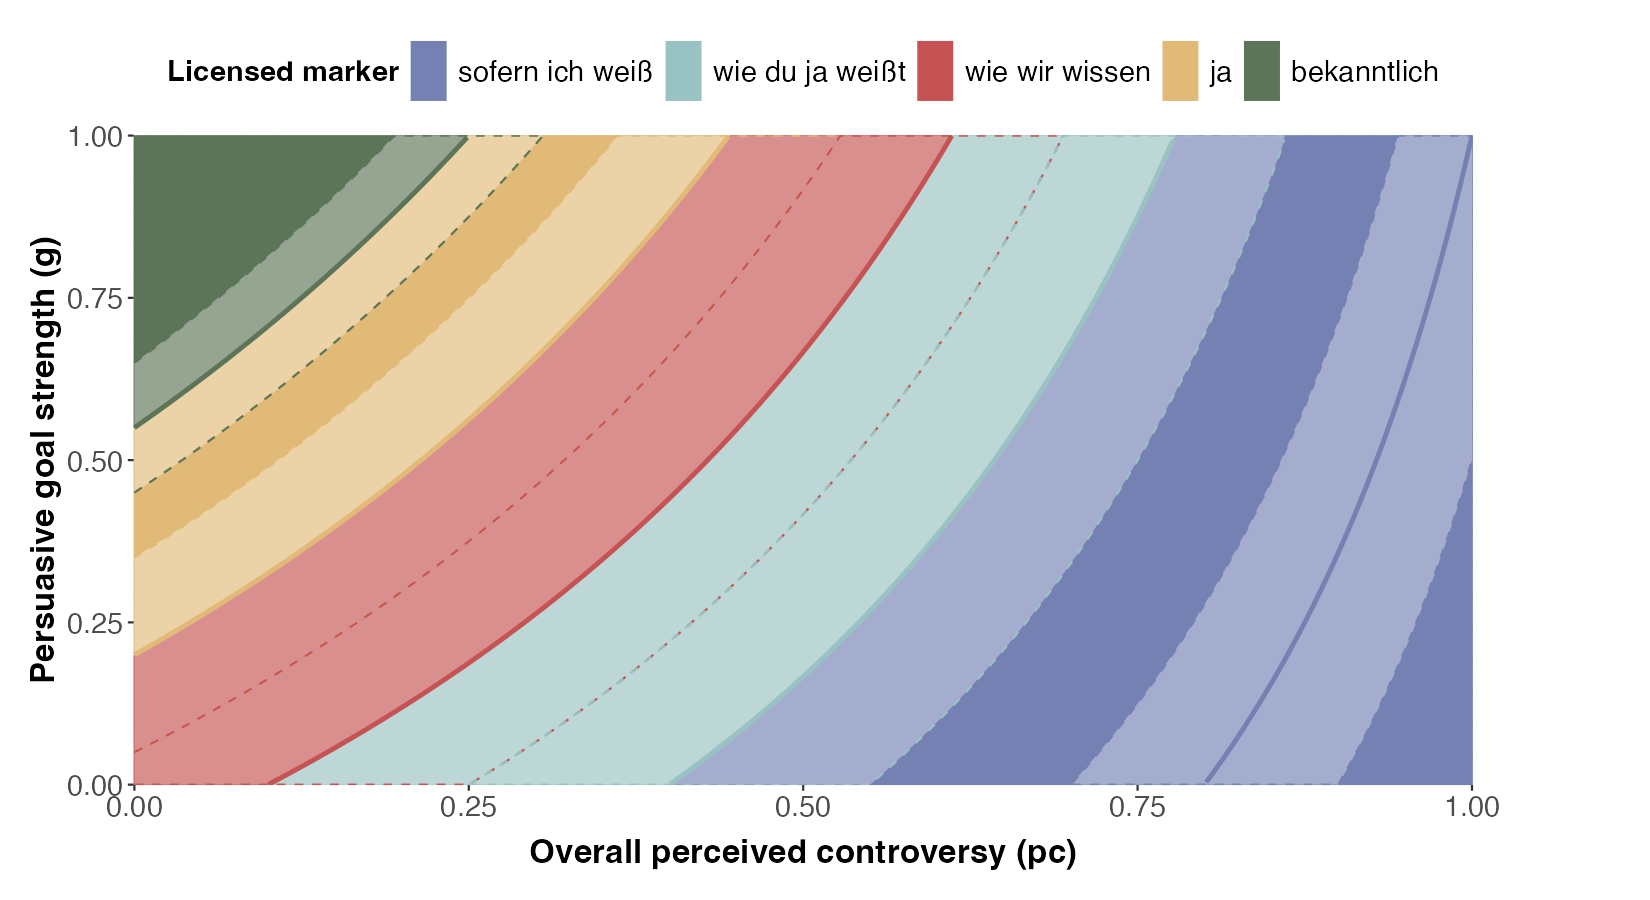
\includegraphics[width=0.65\textwidth]{figures/util_landscape}
  \caption{Utility landscape. Each region is coloured by its licensed marker; solid lines mark mean thresholds $\mu_i$; dashed lines show $\pm\sigma_i$ uncertainty bands.}
  \label{fig:abstract_landscape}
\end{figure}

\begin{figure}[h!]
  \centering
  \begin{subfigure}[b]{0.32\textwidth}
    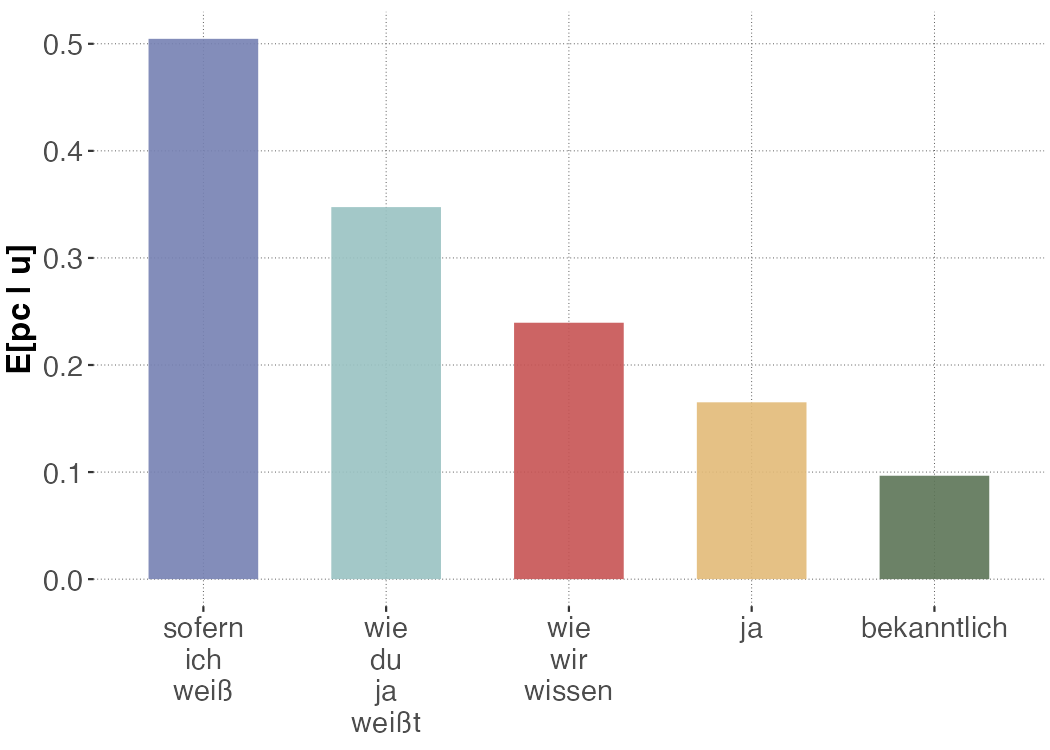
\includegraphics[width=\textwidth]{figures/pc_given_u}
    \caption{$\mathbb{E}[pc \mid u]$}
  \end{subfigure}
  \hfill
  \begin{subfigure}[b]{0.32\textwidth}
    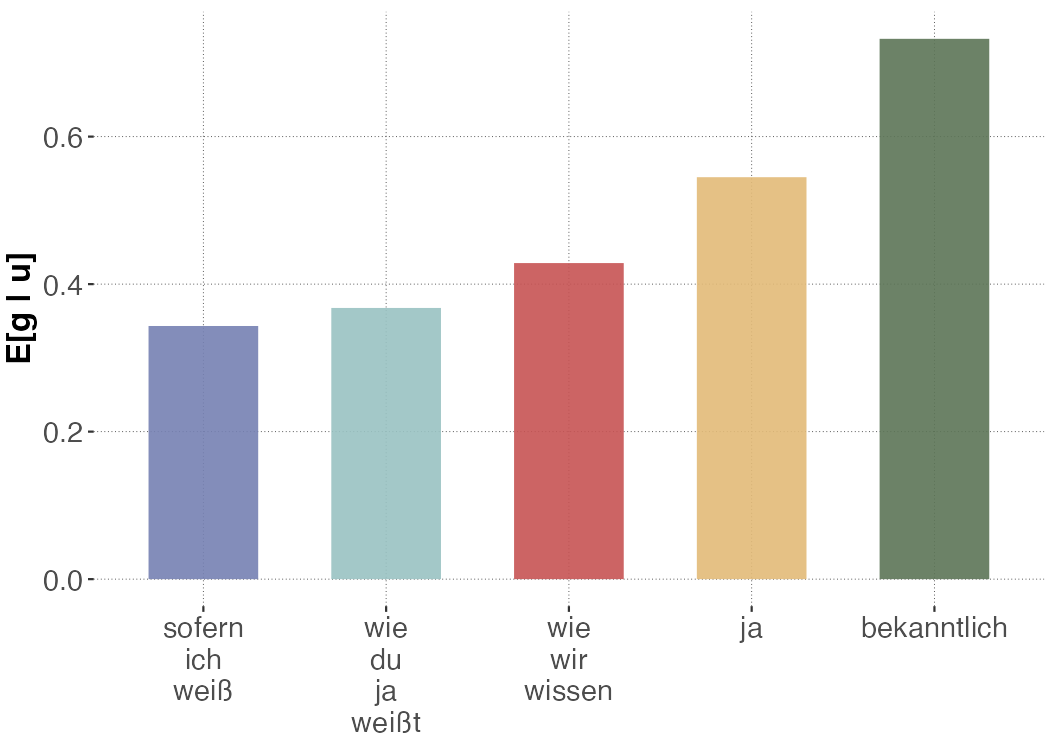
\includegraphics[width=\textwidth]{figures/g_given_u}
    \caption{$\mathbb{E}[g \mid u]$}
  \end{subfigure}
  \hfill
  \begin{subfigure}[b]{0.32\textwidth}
    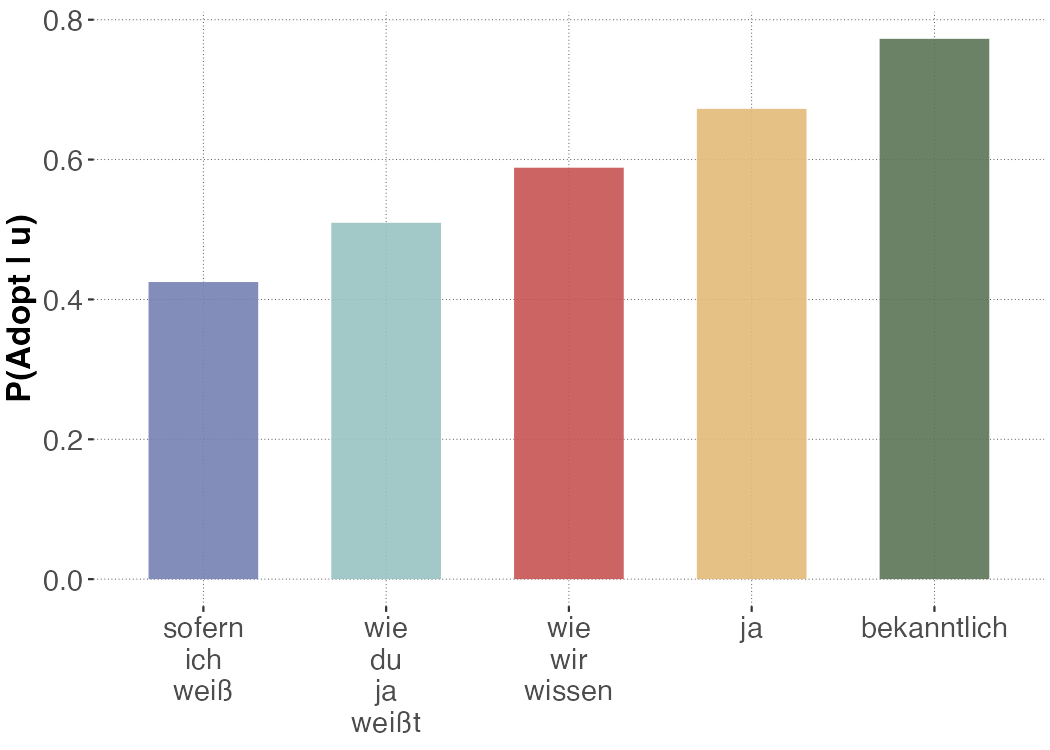
\includegraphics[width=\textwidth]{figures/adopt_given_u}
    \caption{$P(\mathrm{Adopt}(q) \mid u)$}
  \end{subfigure}
  \caption{Core posterior predictions across the five markers. Stronger markers license lower inferred controversy, higher inferred goal strength, and higher adoption probability.}
  \label{fig:abstract_posteriors}
\end{figure}

\textbf{Conclusion \& Outlook.}
We show that the model captures the core intuitions motivated by our opening example: Figures~\ref{fig:abstract_landscape}--\ref{fig:abstract_posteriors} illustrate how the utility landscape partitions marker-licensed regions and how stronger markers shift the posterior toward lower $pc$, higher $g$, and greater adoption likelihood. Beyond these core patterns, the model yields further testable predictions: the interval structure predicts asymmetric infelicity, where strong markers incur larger penalties when used in mismatched contexts than weak markers, which is of interest from a semantic perspective; and credibility discounting, where a sceptical listener with a high prior on $pc$ can detect the manipulative use of a strong marker and withhold adoption, which is of interest from a communicative one. These predictions call for two experiments. A comprehension study would manipulate $pc_{\mathrm{prop}}$ and $pc_{\mathrm{prag}}$ in vignettes, measuring inferred controversy, goal strength, and adoption as a function of marker choice via Bayesian model fitting. A production study would manipulate goal strength and controversy directly, testing whether speakers select stronger markers under higher goals and lower controversy. Together, the two studies close the comprehension--production loop and allow direct estimation of the model's threshold and utility parameters from behavioural data.

\printbibliography
\clearpage
% ══════════════════════════════════════════════════════════════════════════════
\section{Model specification}
% ══════════════════════════════════════════════════════════════════════════════

On the comprehension side, the listener observes an utterance $u$ containing a consensus marker applied to a proposition $p$, followed by a proposed action $q$. The listener performs a joint inference about (i) the speaker's persuasive goal strength $g$ in advancing $q$, and (ii) the perceived controversy $pc$ of $p$, and, as a downstream consequence, about whether to adopt $\mathrm{Adopt}(q)$.

We treat perceived controversy as community-relative and gradient, and decompose it into two components:
$pc_{\text{prop}} \in [0,1]$ (propositional controversy; e.g.\ implausibility relative to world knowledge) and
$pc_{\text{prag}} \in [0,1]$ (pragmatic controversy; e.g.\ expected disagreement / lack of common-ground alignment in the relevant epistemic community).
Overall perceived controversy is computed by a multiplicative interaction function
\begin{equation}
pc \;=\; PC(pc_{\text{prop}}, pc_{\text{prag}})
\;=\;
pc_{\text{prop}} \cdot pc_{\text{prag}},
\end{equation}
so that high propositional controversy can be attenuated by low pragmatic controversy (and vice versa), reflecting the idea that controversy is assessed relative to an epistemic community rather than absolute plausibility alone.

Consensus markers lexicalize thresholds over a utility function:
\begin{equation}
U(pc, g)
\;=\;
- w_{pc} \cdot pc
+
w_g \cdot g
-
w_{\mathrm{int}} \cdot (pc \cdot g),
\label{eq:utility}
\end{equation}
where $w_{pc}, w_g, w_{\mathrm{int}} > 0$. The interaction term $-(w_{\mathrm{int}} \cdot pc \cdot g)$ captures the idea that persuasive effort is increasingly costly when perceived controversy is high: even a speaker with a strong goal $g$ incurs a substantial utility penalty when $pc$ is large, so the optimal strategy is to use a stronger marker only when controversy is genuinely low.

\paragraph{Noisy thresholds.}
Each marker $u_i$ is associated with a lower threshold $\mu_i$ that marks the lower boundary of its licensed utility region. In principle, thresholds could be treated as fixed parameters. However, intuitive plausibility considerations---and the potential for empirical overlap between adjacent markers such as \textit{wie wir wissen} and \textit{ja}---motivate treating each threshold as a latent random variable:
\begin{equation}
\theta_i \;\sim\; \mathcal{N}(\mu_i,\, \sigma_i^2),
\label{eq:noisy_threshold}
\end{equation}
where $\mu_i$ is the mean (expected) threshold and $\sigma_i \geq 0$ controls how diffuse or overlapping marker boundaries are. When $\sigma_i \to 0$ the model recovers a hard boundary; larger $\sigma_i$ allows adjacent markers to share utility regions, modelling graded speaker variation or genuine lexical ambiguity between near-synonymous markers.

A marker is felicitous when $U$ falls within the interval $[\theta_i, \theta_{i+1})$. Taking the expectation over independently drawn $\theta_i$ and $\theta_{i+1}$, the likelihood factorises:
\begin{equation}
P(u_i \mid pc, g)
\;\propto\;
\mathbb{E}_{\theta_i}\!\left[\sigma\!\bigl(\lambda\,(U - \theta_i)\bigr)\right]
\;\cdot\;
\mathbb{E}_{\theta_{i+1}}\!\left[\sigma\!\bigl(-\lambda\,(U - \theta_{i+1})\bigr)\right],
\label{eq:likelihood}
\end{equation}
where $\sigma(x) = (1+e^{-x})^{-1}$ is the logistic function and $\lambda > 0$ controls the sharpness of the interval boundaries. Each expectation is a logistic-normal integral. Applying the standard probit approximation
\[
\mathbb{E}_{t \sim \mathcal{N}(\mu,\sigma^2)}\!\left[\sigma(a(U-t))\right]
\;\approx\;
\Phi\!\left(\frac{a\,(U-\mu)\,c}{\sqrt{1+(a\sigma c)^2}}\right),
\]
where $\Phi$ is the standard normal CDF and $c = \sqrt{\pi/8}$, yields the closed-form likelihood:
\begin{equation}
P(u_i \mid pc, g)
\;\propto\;
\underbrace{\Phi\!\!\left(\frac{\lambda\,(U-\mu_i)\,c}{\sqrt{1+(\lambda\sigma_i c)^2}}\right)}_{\text{lower bound: }U \geq \theta_i}
\;\cdot\;
\underbrace{\Phi\!\!\left(\frac{-\lambda\,(U-\mu_{i+1})\,c}{\sqrt{1+(\lambda\sigma_{i+1} c)^2}}\right)}_{\text{upper bound: }U < \theta_{i+1}},
\label{eq:likelihood_noisy}
\end{equation}
where the second factor is set to 1 for the strongest marker ($\mu_{i+1} = +\infty$). The approximation error is below $0.01$ across the parameter range of interest. This formulation ensures that each $(pc, g)$ point preferentially licenses the marker whose mean threshold $\mu_i$ best matches the current utility level, while $\sigma_i$ controls how sharply or diffusely that licensing is defined.

%\begin{remark}
%A one-sided likelihood of the form $P(u \mid pc, g) \propto \exp(\lambda(U - \theta_u))$ is not suitable here. Because $\theta_u$ enters only as a constant additive shift in log-space, it factors out of the normalising sum and cancels, rendering the posterior $P(pc, g \mid u)$ identical across all markers and equal to the prior. The interval formulation in Eq.~\eqref{eq:likelihood_noisy} avoids this degeneracy by making each marker's likelihood explicitly dependent on the local value of $U(pc,g)$ relative to both its own mean threshold and that of the adjacent stronger marker.
%\end{remark}

The mean thresholds are ordered by marker strength:
\[
\mu_{\textit{sofern ich weiß}}
\;<\;
\mu_{\textit{wie du ja weißt}}
\;<\;
\mu_{\textit{wie wir wissen}}
\;<\;
\mu_{\textit{ja}}
\;<\;
\mu_{\textit{bekanntlich}},
\]
so that stronger markers require higher utility in expectation to be felicitous. Adjacent markers with similar $\mu$ values and large $\sigma$ will exhibit overlapping licensed regions, predicting variable or context-dependent use for those pairs. Figure~\ref{fig:util_landscape} illustrates the utility landscape: each region of the $(pc, g)$ plane is coloured by its licensed marker under default parameters, with threshold boundaries and their $\pm\sigma$ uncertainty bands superimposed.

\paragraph{Posterior inference.}
Upon observing $u_i$, the listener inverts this mapping via Bayes' theorem:
\begin{equation}
P(pc_{\text{prop}}, pc_{\text{prag}}, g \mid u_i)
\;\propto\;
P(u_i \mid PC(pc_{\text{prop}}, pc_{\text{prag}}), g)\,
P(pc_{\text{prop}})\,P(pc_{\text{prag}})\,P(g),
\label{eq:posterior}
\end{equation}
where we adopt uniform priors $P(pc_{\text{prop}}), P(pc_{\text{prag}}), P(g) \sim \mathrm{Uniform}[0,1]$ as the default.

Action adoption is modelled as a downstream decision based on the posterior:
\begin{equation}
P(\mathrm{Adopt}(q) \mid u)
= \iiint
\sigma(\eta_0 + \eta_g g - \eta_{pc}\, pc - \eta_{\mathrm{int}}\, g \cdot pc)
\; P(pc_{\mathrm{prop}}, pc_{\mathrm{prag}}, g \mid u)
\; dpc_{\mathrm{prop}}\, dpc_{\mathrm{prag}}\, dg,
\label{eq:adoption}
\end{equation}
where $\eta_g, \eta_{pc}, \eta_{\mathrm{int}} > 0$. The interaction term $-\eta_{\mathrm{int}}\, g \cdot pc$ penalises high persuasive intent when controversy is high, enabling the reversal of adoption order under scepticism.

% ══════════════════════════════════════════════════════════════════════════════
\section{Qualitative model predictions}
% ══════════════════════════════════════════════════════════════════════════════

The comprehension model predicts systematic inferences about perceived controversy and speaker goal strength from the observed marker, and downstream effects on action adoption. Figures~\ref{fig:predictions}--\ref{fig:discounting} summarise these predictions, derived from Eq.~\eqref{eq:likelihood_noisy}--\eqref{eq:adoption} under default parameters ($\lambda=6$, $w_{pc}=w_g=1$, $w_{\mathrm{int}}=0.8$, $\eta_g=\eta_{pc}=2$).

% ── Figure: utility landscape ─────────────────────────────────────────────────

\begin{figure}[h!]
  \centering
  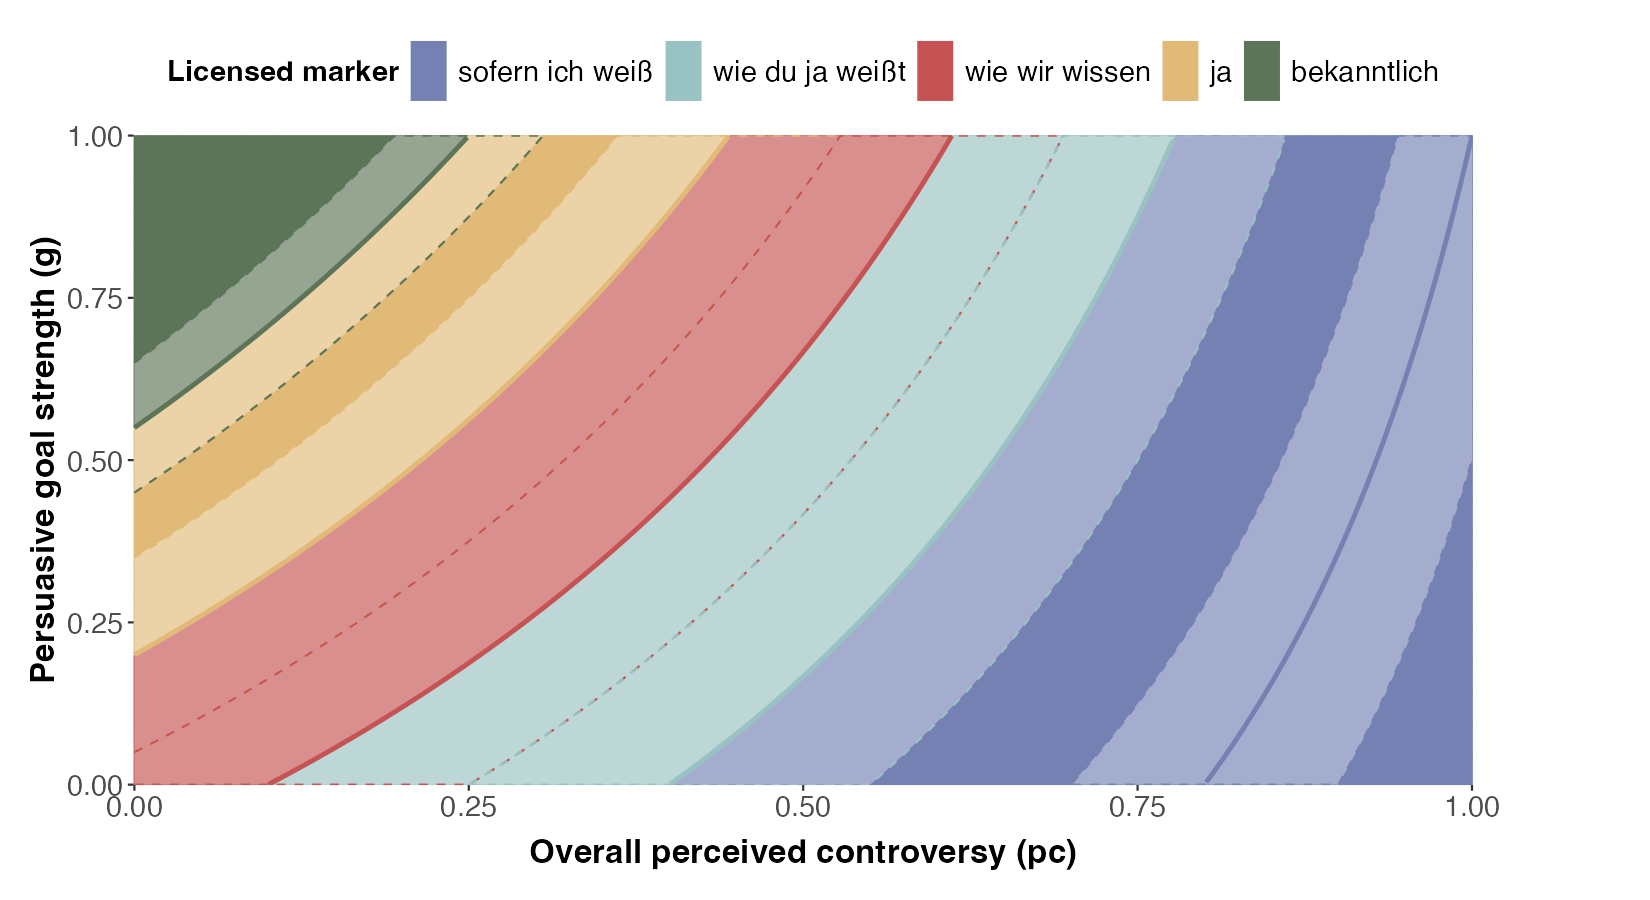
\includegraphics[width=0.85\textwidth]{figures/util_landscape}
  \caption{%
    Utility landscape $U(pc, g)$ under default parameters. Each region of the
    $(pc, g)$ plane is filled with the colour of the marker licensed there
    (i.e., the marker whose mean threshold interval $[\mu_i, \mu_{i+1})$ contains
    the utility value at that point). Solid lines mark the mean threshold
    boundaries $\mu_i$; dashed lines show the $\pm\sigma_i$ uncertainty bands.
    The white semi-transparent ribbons between dashed lines indicate the
    overlap zones in which adjacent markers compete. The gradient from lower-left
    (low utility; weak markers licensed) to upper-right (high utility; strong
    markers licensed) reflects the joint effect of decreasing controversy and
    increasing goal strength on the speaker's utility.
  }
  \label{fig:util_landscape}
\end{figure}

% ── Figure: three core posteriors ─────────────────────────────────────────────

\begin{figure}[h!]
  \centering
  \begin{subfigure}[b]{0.32\textwidth}
    \centering
    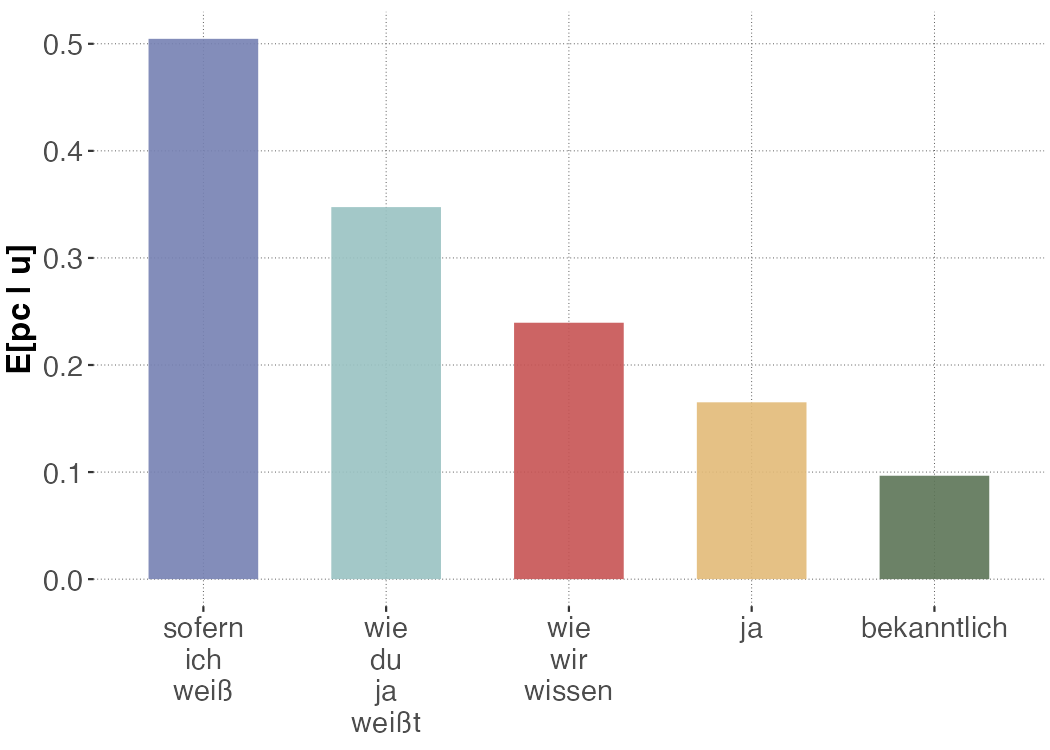
\includegraphics[width=\textwidth]{figures/pc_given_u}
    \caption{$\mathbb{E}[pc \mid u]$ per marker.}
    \label{fig:pred_pc}
  \end{subfigure}
  \hfill
  \begin{subfigure}[b]{0.32\textwidth}
    \centering
    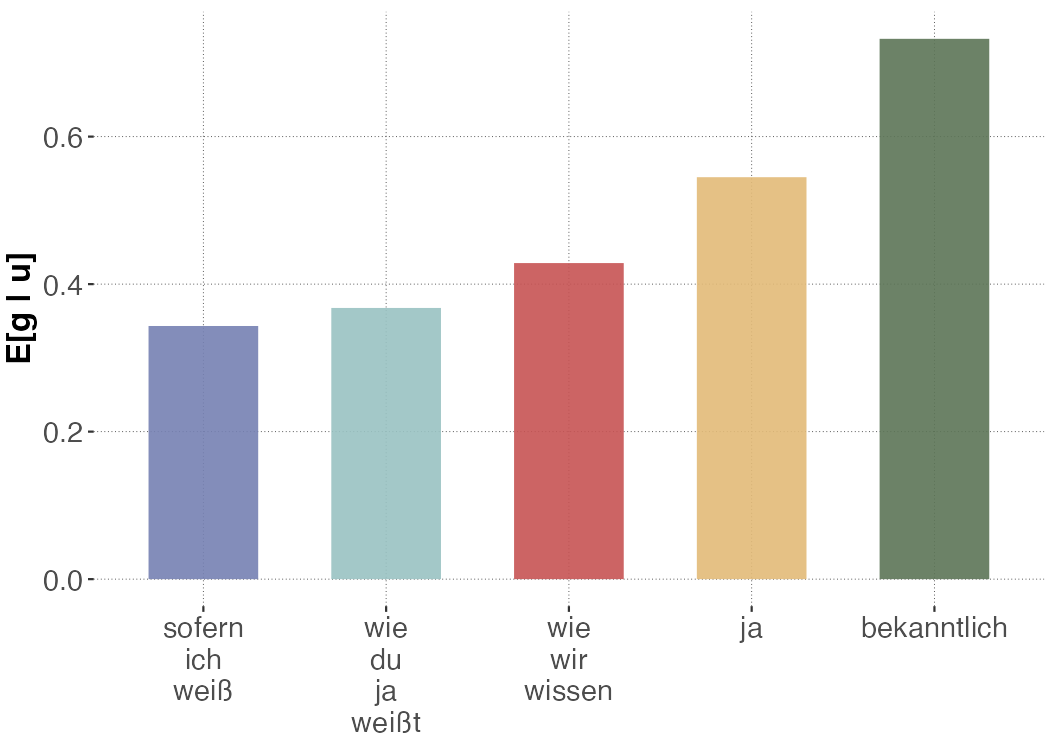
\includegraphics[width=\textwidth]{figures/g_given_u}
    \caption{$\mathbb{E}[g \mid u]$ per marker.}
    \label{fig:pred_g}
  \end{subfigure}
  \hfill
  \begin{subfigure}[b]{0.32\textwidth}
    \centering
    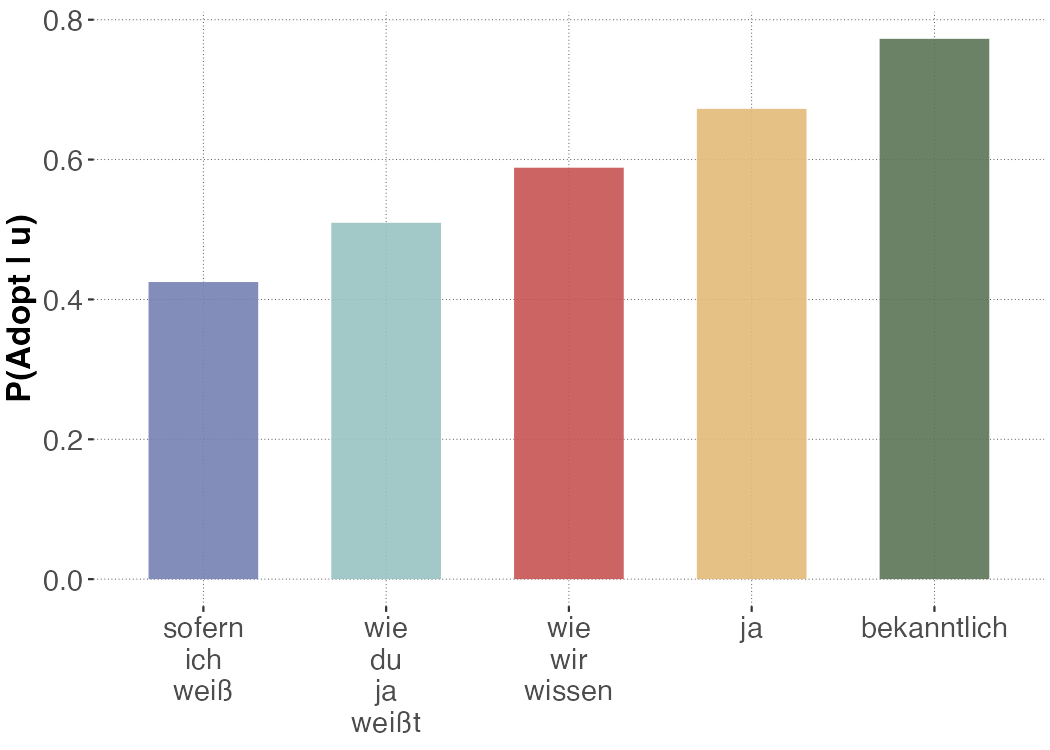
\includegraphics[width=\textwidth]{figures/adopt_given_u}
    \caption{$P(\mathrm{Adopt}(q) \mid u)$ per marker.}
    \label{fig:pred_adopt}
  \end{subfigure}
  \caption{%
    Core posterior summaries for the five consensus markers ordered by strength.
    \textbf{(a)}~Posterior expected perceived controversy $\mathbb{E}[pc\mid u]$
    decreases monotonically with marker strength.
    \textbf{(b)}~Posterior expected persuasive goal strength $\mathbb{E}[g\mid u]$
    increases monotonically.
    \textbf{(c)}~Downstream adoption probability $P(\mathrm{Adopt}(q)\mid u)$
    increases monotonically under default adoption weights.
    All panels are computed by grid-approximated Bayesian inference under
    Eq.~\eqref{eq:likelihood_noisy} with uniform priors.
  }
  \label{fig:predictions}
\end{figure}
% ══════════════════════════════════════════════════════════════════════════════
\textbf{Marker strength and perceived controversy.}
% ══════════════════════════════════════════════════════════════════════════════
Because stronger markers are licensed only when the utility $U(pc,g)$ exceeds a higher mean threshold, observing a stronger marker shifts the listener's posterior toward lower overall $pc$:
\[
\mathbb{E}[pc \mid u=\textit{bekanntlich}]
\;<\;
\mathbb{E}[pc \mid u=\textit{ja}]
\;<\;\cdots\;<\;
\mathbb{E}[pc \mid u=\textit{sofern ich wei\ss}].
\]
In particular, stronger markers bias the listener towards interpretations in which $p$ is sufficiently settled in the relevant community (Figure~\ref{fig:pred_pc}).
% ══════════════════════════════════════════════════════════════════════════════
\textbf{Marker strength and persuasive goal strength.}
% ══════════════════════════════════════════════════════════════════════════════
Because utility increases with $g$, observing a stronger marker shifts posterior mass toward higher goal strength:
\[
\mathbb{E}[g \mid u=\textit{bekanntlich}]
\;>\;
\mathbb{E}[g \mid u=\textit{ja}]
\;>\;\cdots\;>\;
\mathbb{E}[g \mid u=\textit{sofern ich wei\ss}].
\]
Consensus markers thus trigger theory-of-mind inferences about the speaker's intention to push the addressee toward adopting $q$ (Figure~\ref{fig:pred_g}).
% ══════════════════════════════════════════════════════════════════════════════
\textbf{Downstream action adoption.}
% ══════════════════════════════════════════════════════════════════════════════
Since adoption increases with $g$ and decreases with $pc$ in Eq.~\eqref{eq:adoption}, $P(\mathrm{Adopt}(q)\mid u)$ is predicted to be highest for strong markers when overall controversy is low, and moderated when controversy is high. Because marker strength jointly affects inferred $pc$ and $g$, the model predicts (i) higher adoption for stronger markers in low-controversy contexts, and (ii) a characteristic dissociation under high controversy: strong markers may still increase perceived persuasive pressure while willingness to act remains limited by high $pc$ (Figure~\ref{fig:pred_adopt}).

% ── Figure: decomposition heatmaps ────────────────────────────────────────────

\begin{figure}[h!]
  \centering
  \begin{subfigure}[b]{0.48\textwidth}
    \centering
    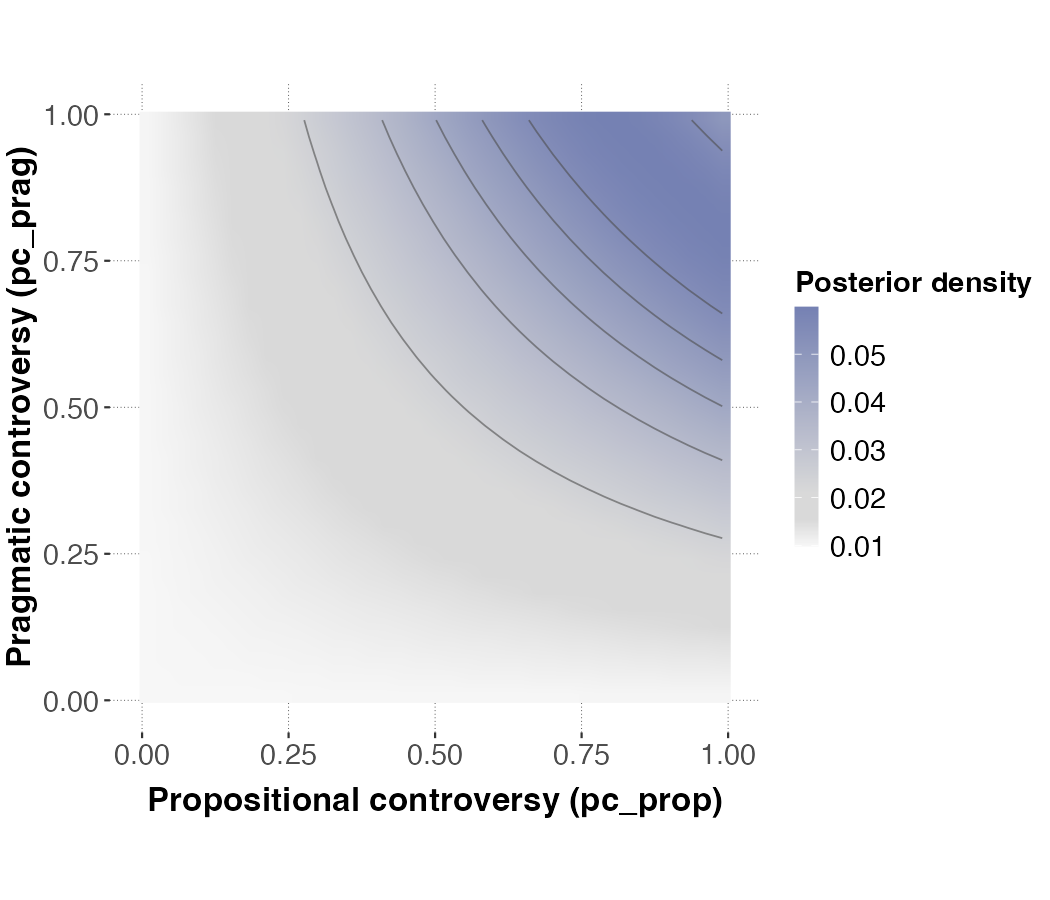
\includegraphics[width=\textwidth]{figures/int_pc_prop_pc_prag_weak}
    \caption{Weak marker: \textit{sofern ich wei\ss}.}
    \label{fig:decomp_weak}
  \end{subfigure}
  \hfill
  \begin{subfigure}[b]{0.48\textwidth}
    \centering
    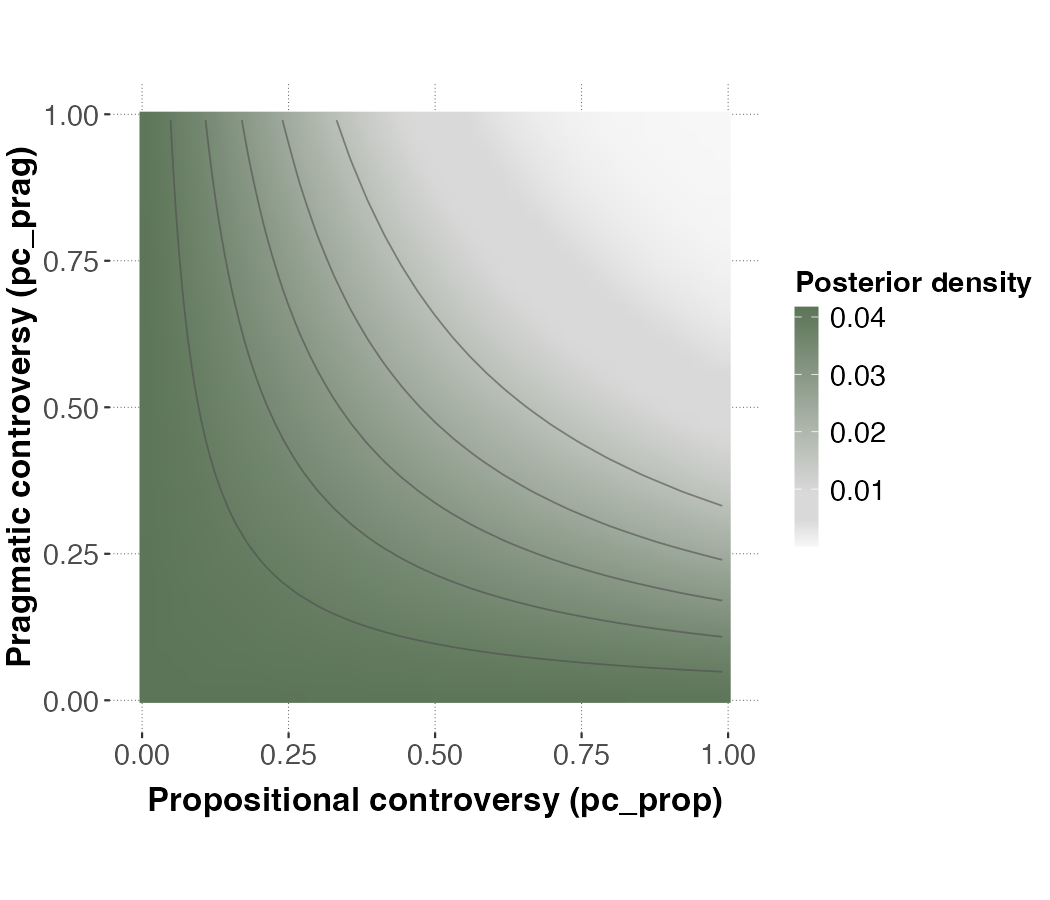
\includegraphics[width=\textwidth]{figures/int_pc_prop_pc_prag_strong}
    \caption{Strong marker: \textit{bekanntlich}.}
    \label{fig:decomp_strong}
  \end{subfigure}
  \caption{%
    Marginal posterior $P(pc_{\text{prop}}, pc_{\text{prag}} \mid u)$, obtained by
    integrating out $g$, for the weakest and strongest markers.
    \textbf{(a)}~For \textit{sofern ich wei\ss}, posterior mass concentrates
    where both components are high, consistent with a genuinely controversial
    proposition.
    \textbf{(b)}~For \textit{bekanntlich}, mass shifts toward low
    $pc_{\text{prop}}$; $pc_{\text{prag}}$ remains relatively unconstrained,
    because $pc_{\text{prop}} \approx 0$ alone collapses overall controversy
    regardless of $pc_{\text{prag}}$.
    This asymmetry reflects the compensation structure of $pc = pc_{\text{prop}}
    \cdot pc_{\text{prag}}$: strong markers can be licensed equally by
    propositional plausibility or community alignment, and listeners trade off
    these sources in interpretation.
  }
  \label{fig:decomp}
\end{figure}
% ══════════════════════════════════════════════════════════════════════════════
\paragraph{Decomposition of propositional and pragmatic controversy.}
% ══════════════════════════════════════════════════════════════════════════════
Since $pc = pc_{\text{prop}} \cdot pc_{\text{prag}}$, the model predicts a characteristic compensation pattern: high propositional controversy can be ``rescued'' by low pragmatic controversy (high community alignment), yielding low overall $pc$. The same marker can therefore be licensed by either factual plausibility or strong community alignment, and listeners trade off these sources in interpreting the utterance. Figure~\ref{fig:decomp} contrasts the marginal posteriors over $(pc_{\text{prop}}, pc_{\text{prag}})$ for the weakest and strongest markers.

% ── Figure: super-additivity interaction plot ─────────────────────────────────
\begin{comment}
\begin{figure}[h!]
  \centering
  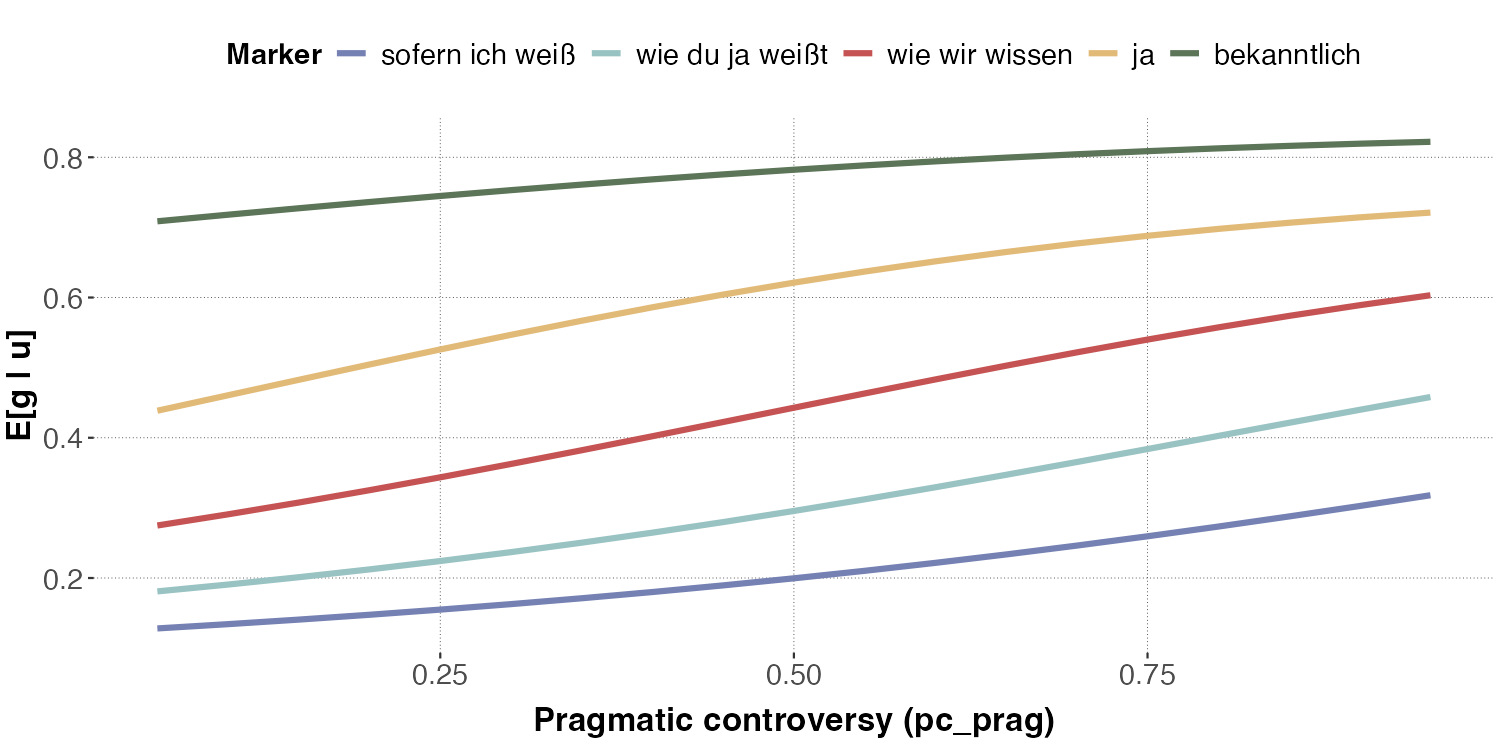
\includegraphics[width=0.92\textwidth]{figures/int_pc_marker_g}
  \caption{%
    Super-additive interaction between marker strength and pragmatic controversy
    in inferred goal strength. Each line shows $\mathbb{E}[g\mid u, pc_{\text{prag}}]$
    for one marker as $pc_{\text{prag}}$ varies (with $pc_{\text{prop}}$ fixed at $0.5$).
    The gap between strong and weak markers widens as $pc_{\text{prag}}$ increases,
    reflecting the interaction term $-(w_{\mathrm{int}} \cdot pc \cdot g)$ in the
    utility function: in high-controversy contexts, only a strong marker can
    credibly signal sufficient $g$, amplifying the marker-strength effect on
    goal inference.
  }
  \label{fig:superadd}
\end{figure}
% ══════════════════════════════════════════════════════════════════════════════
%\paragraph{Super-additivity of goal inference under controversy.}
% ══════════════════════════════════════════════════════════════════════════════
Because the utility includes the interaction term $-(w_{\mathrm{int}} \cdot pc \cdot g)$, the effect of controversy on inferred goal strength is super-additive: under higher inferred $pc$, observing a strong marker forces a stronger increase in inferred $g$ to place the utterance within the marker's licensed utility interval. The model therefore predicts the largest shifts in $\mathbb{E}[g \mid u]$ for strong markers in high-controversy contexts. Figure~\ref{fig:superadd} illustrates this: lines for strong markers diverge from those for weak markers as $pc_{\text{prag}}$ rises.
\end{comment}
% ── Figure: scalar implicature ────────────────────────────────────────────────
\begin{comment}
\begin{figure}[h!]
  \centering
  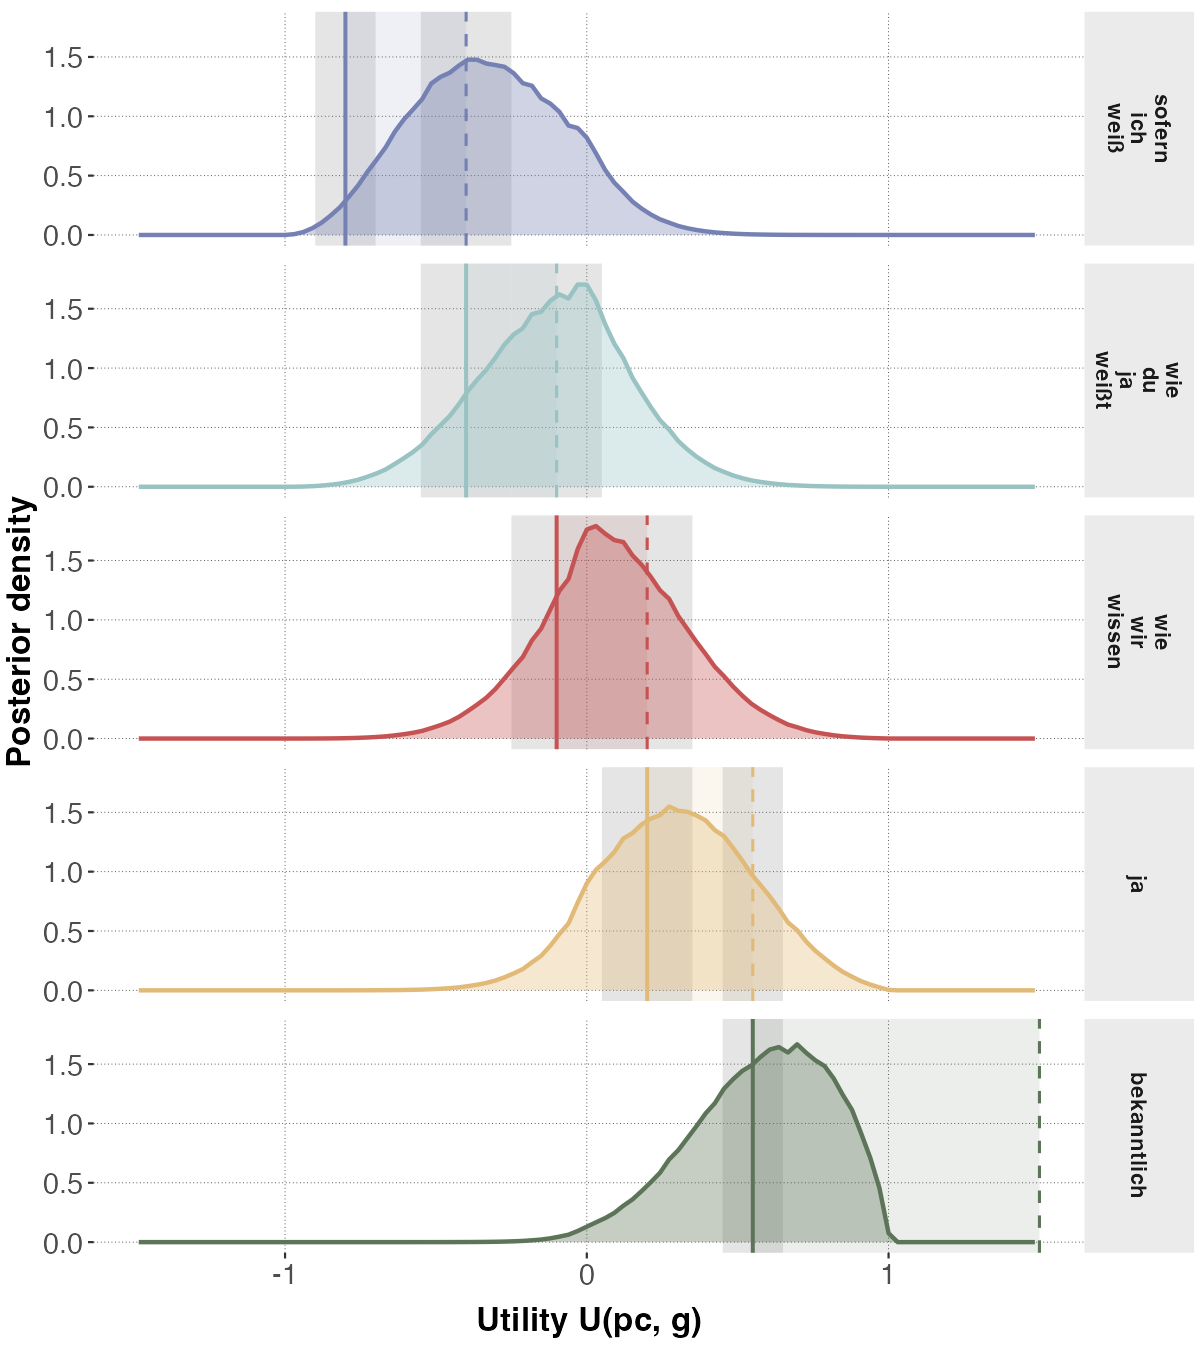
\includegraphics[width=0.5\textwidth]{figures/scalar_implicature.png}
  \caption{%
    Scalar implicature analog. Each panel shows the marginal posterior density
    over utility $P(U \mid u_i)$ for one marker (obtained by integrating out
    $pc_{\text{prop}}, pc_{\text{prag}}, g$). The coloured background rectangle
    marks the licensed interval $[\mu_i, \mu_{i+1})$; the solid vertical line
    marks the marker's own lower threshold $\mu_i$; the dashed line marks the
    upper threshold $\mu_{i+1}$ (the lower boundary of the next stronger marker).
    Grey bands at each boundary indicate the $\pm\sigma$ overlap zone in which
    adjacent markers compete. Posterior mass falls off sharply above $\mu_{i+1}$,
    implementing a scalar implicature: use of $u_i$ implicates that the context
    was insufficiently strong to license the next stronger marker, so the upper
    threshold functions as an implicated upper bound on $U$.
  }
  \label{fig:scalar}
\end{figure}
% ══════════════════════════════════════════════════════════════════════════════

%\paragraph{Scalar implicature analog.}
% ══════════════════════════════════════════════════════════════════════════════
The interval licensing structure generates a scalar implicature analog. Use of a weaker marker $u_i$ implicates that the speaker judged the context utility $U(pc,g)$ insufficient to license the next stronger marker $u_{i+1}$: had it been sufficient, the speaker would have used $u_{i+1}$ (by a Gricean quantity reasoning applied to the scale). The model implements this directly: the posterior over utility $P(U \mid u_i)$ concentrates in $[\mu_i, \mu_{i+1})$ and falls off sharply above $\mu_{i+1}$. The upper threshold thus functions as an implicated upper bound analogous to the `not all' implicature from `some'. Figure~\ref{fig:scalar} illustrates this for each marker in the scale. Crucially, the overlap zones (grey $\pm\sigma$ bands) predict that the implicature is defeasible in proportion to $\sigma_i$: markers with larger noise $\sigma$ generate weaker, more cancellable upper-bound inferences.
\end{comment}

% ── Figure: infelicity ────────────────────────────────────────────────────────

\begin{figure}[h!]
  \centering
  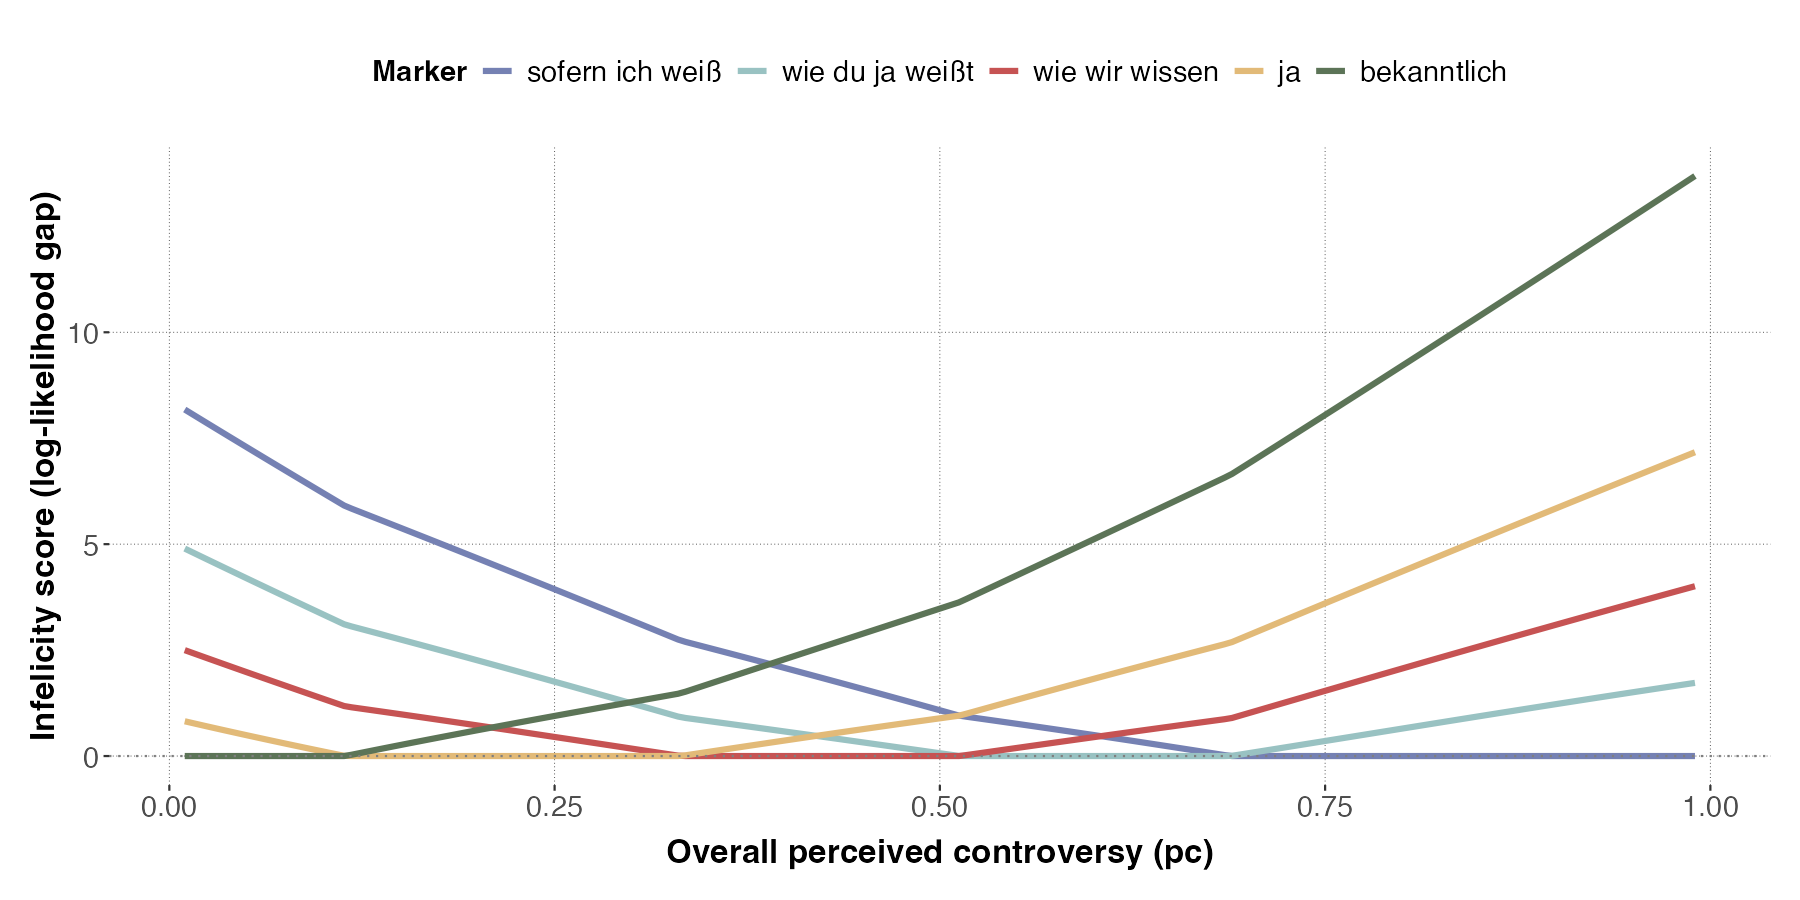
\includegraphics[width=0.6\textwidth]{figures/infelicity.png}
  \caption{%
    Marker-context infelicity scores. Each line shows the infelicity score
    $\log P(u^* \mid pc, g) - \log P(u_i \mid pc, g)$ for one marker as a
    function of $pc$ (with $g$ fixed at $0.7$), where $u^*$ denotes the
    utility-maximising marker at each point. A score of zero means the
    chosen marker is optimal; positive values indicate contextual mismatch.
    The bold line highlights the selected marker; faint lines show all others
    for reference. The asymmetry predicted by the model is visible: using
    \textit{bekanntlich} in high-controversy contexts (large $pc$) incurs a
    sharply rising penalty, whereas using \textit{sofern ich wei\ss} in
    low-controversy contexts incurs only a modest one. This reflects the
    larger utility gap at the strong end of the scale.
  }
  \label{fig:infelicity}
\end{figure}
% ══════════════════════════════════════════════════════════════════════════════
\paragraph{Marker-context mismatch and infelicity.}
% ══════════════════════════════════════════════════════════════════════════════
The interval model assigns a natural infelicity score to any (marker, context) pair: the log-likelihood gap between the optimal marker and the chosen one,
\[
\mathrm{Infelicity}(u_i, pc, g)
\;=\;
\log P(u^* \mid pc, g) - \log P(u_i \mid pc, g)
\;\geq\; 0,
\]
where $u^* = \arg\max_{u_j} P(u_j \mid pc, g)$. The model predicts asymmetric pragmatic oddness: using \textit{bekanntlich} in a genuinely contested context incurs a larger infelicity penalty than using \textit{sofern ich wei\ss} in a clearly settled one, because the utility gap is larger at the strong end of the scale. Figure~\ref{fig:infelicity} illustrates this: the infelicity curve for strong markers rises sharply with $pc$, while that for weak markers rises only gradually.

% ── Figure: credibility discounting ──────────────────────────────────────────

\begin{figure}[h!]
  \centering
  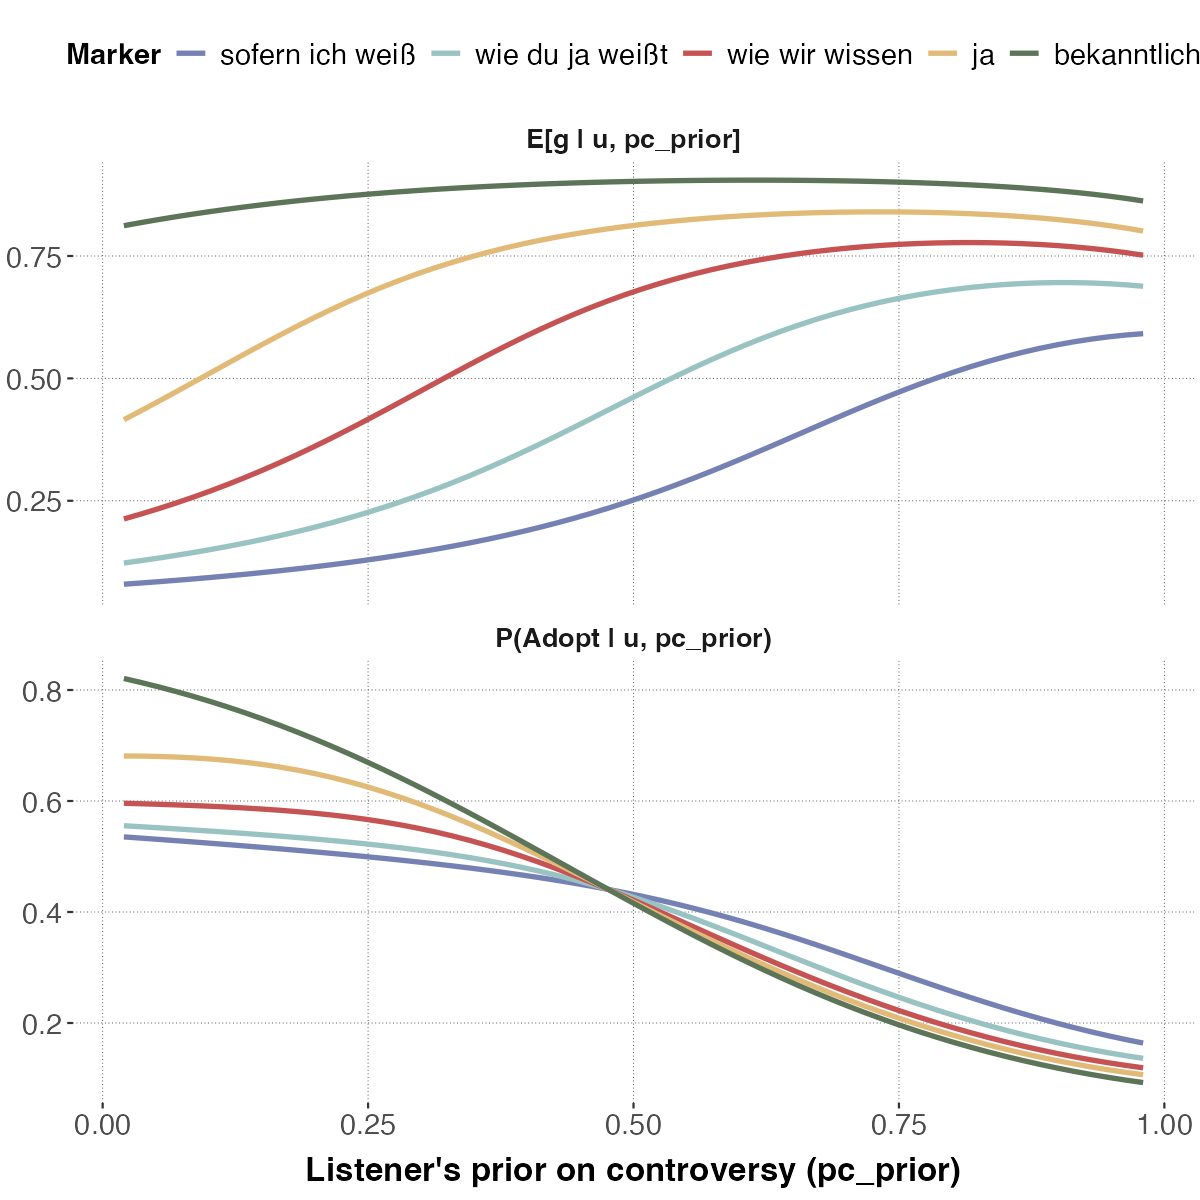
\includegraphics[width=0.6\textwidth]{figures/credibility_discounting.png}
  \caption{%
    Credibility discounting under scepticism. Both panels show quantities as a
    function of the listener's independent prior belief $pc_{\text{prior}}$ about
    how controversial the topic is. \textbf{Top:} $\mathbb{E}[g \mid u, pc_{\text{prior}}]$
    for each marker---lines remain stably ordered, showing that the marker
    reliably signals goal strength regardless of the listener's controversy
    belief. \textbf{Bottom:} $P(\mathrm{Adopt}(q) \mid u, pc_{\text{prior}})$,
    modelling a listener who fixes $pc = pc_{\text{prior}}$ and applies an
    interaction penalty $-\eta_{\text{int}} \cdot g \cdot pc_{\text{prior}}$ that
    penalises high persuasive intent when the topic is known to be contested.
    As $pc_{\text{prior}}$ rises, adoption lines first converge and then cross:
    strong markers, which signal high $g$, incur a disproportionate penalty and
    eventually fall below weak markers in adoption probability. The dissociation
    between the two panels captures the core prediction---goal inference stays
    ordered while adoption reverses---reflecting the communicative risk of
    deploying a strong consensus marker on a genuinely controversial topic.
  }
  \label{fig:discounting}
\end{figure}
% ══════════════════════════════════════════════════════════════════════════════
\paragraph{Credibility discounting under scepticism.}
% ══════════════════════════════════════════════════════════════════════════════
A skeptical listener may have an independent prior belief $pc_{\text{prior}}$ about how controversial the topic is---for instance, because they know it from world knowledge---and weight this prior over the marker's signal about $pc$. In the limit of full skepticism, the listener uses $pc_{\text{prior}}$ directly in the adoption equation rather than the marker-informed posterior over $pc$. This produces a characteristic dissociation: $\mathbb{E}[g \mid u, pc_{\text{prior}}]$ remains monotonically ordered with marker strength (the $g$-signal is still received), but $P(\mathrm{Adopt}(q) \mid u, pc_{\text{prior}})$ is modulated by an interaction term $-\eta_{\text{int}} \cdot g \cdot pc_{\text{prior}}$, which penalises high persuasive intent precisely when the topic is known to be contested. Since stronger markers signal higher $g$, they incur a larger penalty at high $pc_{\text{prior}}$, producing a reversal: what reads as strong commitment in a low-controversy context is reinterpreted as suspicious over-assertiveness in a high-controversy one. Figure~\ref{fig:discounting} illustrates this: the top panel (goal inference) stays ordered at all values of $pc_{\text{prior}}$, while the bottom panel (adoption) shows lines first converging and then crossing at sufficiently high $pc_{\text{prior}}$ and $\eta_{\text{int}}$. The model thus predicts not merely an erosion but a genuine reversal of adoption order for sceptical listeners---a communicative regime where the manipulative use of strong markers backfires.

% ══════════════════════════════════════════════════════════════════════════════
\section{Experiments}
% ══════════════════════════════════════════════════════════════════════════════

We test the comprehension--production connection implied by the model: (i) listeners infer perceived controversy and speaker goal strength from a consensus marker and use these in downstream action decisions; (ii) speakers choose markers as a function of inferred controversy and persuasive goal strength.

\subsection{General materials and factors}

\paragraph{Markers.}
The utterance $u$ contains one of five consensus markers (German):
\[
u \in \{\textit{sofern ich weiß},\ \textit{wie du ja weißt},\ \textit{wie wir wissen},\ \textit{ja},\ \textit{bekanntlich}\},
\]
assumed to lexicalize increasing mean thresholds $\mu_u$.

\paragraph{Proposition and action.}
Each item consists of a proposition $p$ (an informational claim) and a proposed action $q$ (a concrete recommendation). The target sentence frame is:
\[
\text{MARKER}(p)\ \ \Rightarrow\ \ \text{therefore adopt } q.
\]
Example (schematic):
\begin{quote}
\small
\textit{Bekanntlich} $p$ (``Xeliherb ist assoziiert mit Ralocrop.''). Therefore, $q$ (``Wir sollten Ralocrop auch anbauen''). (See Exp. 2 in \citet{lassiter2024rationality})
\end{quote}

\paragraph{Manipulating controversy.}
We manipulate two sources of perceived controversy:
\begin{itemize}
\item \textbf{Propositional controversy} ($pc_{\text{prop}}$): plausibility/compatibility with world knowledge and evidence strength (e.g.\ strong vs.\ weak evidence; plausible vs.\ surprising claim).
\item \textbf{Pragmatic controversy} ($pc_{\text{prag}}$): expected disagreement / common-ground alignment in a specified community (e.g.\ shared expert consensus vs.\ polarized community).
\end{itemize}

\noindent Each item is paired with short contextual information implementing a $2 \times 2$ manipulation:
\[
pc_{\text{prop}} \in \{\text{low},\text{high}\}
\quad\times\quad
pc_{\text{prag}} \in \{\text{low},\text{high}\}.
\]
This directly targets the model decomposition $pc = pc_{\text{prop}}\cdot pc_{\text{prag}}$.

\paragraph{Norming study.}
We can use norming studies to elicit human prior to context manipulations that selectively affect (i) plausibility/evidence ($pc_{\text{prop}}$) and (ii) expected disagreement/community alignment ($pc_{\text{prag}}$).

% ==========================================================
\subsection{Experiment 1: Comprehension (joint inference and decision making)}

\paragraph{Goal.}
Test the listener-side predictions:
(i) marker strength drives inferences about $pc$ and $g$;
(ii) decomposition trade-off between $pc_{\text{prop}}$ and $pc_{\text{prag}}$;
(iii) downstream effects on $\Pr(\mathrm{Adopt}(q)\mid u)$.

\paragraph{Design.}
A mixed factorial design:
\begin{itemize}
\item \textbf{Within-participant factor:} marker $u$ (5 levels).
\item \textbf{Within-participant factor:} contextual manipulations $pc_{\text{prop}}$ (\textit{high} vs. \textit{low}) and $pc_{\text{prag}}$ (\textit{high} vs. \textit{low}).
\end{itemize}
We use a Latin-square scheme so each participant sees each \emph{item} in exactly one marker condition (to avoid direct within-item comparisons of markers), while still seeing all factor levels across items.

\paragraph{Materials.}
Each trial shows:
\begin{enumerate}
\item a short vignette specifying an epistemic community $C$ (e.g.\ ``students in your department'', ``medical experts'', ``local residents''),
\item two context sentences implementing $pc_{\text{prop}}$ and $pc_{\text{prag}}$ (evidence strength vs.\ community alignment),
\item the target message: marker-applied claim $p$ followed by recommended action $q$.
\end{enumerate}

\paragraph{Procedure.}
For each trial, participants read the vignette and target message, then answer:
\begin{enumerate}
\item \textbf{Adoption decision}
\[
\text{Would you adopt } q?\ \ (\text{yes/no}) \quad\text{or}\quad \text{slider }[0,100].
\]
\item \textbf{Joint inference}
\begin{itemize}
\item perceived overall controversy:
\[
\widehat{pc}\ \text{(``How controversial is $p$ in community $C$?'')} \in [0,100]
\]
\item perceived speaker goal strength:
\[
\widehat{g}\ \text{(``How strongly is the speaker trying to persuade you to do $q$?'')} \in [0,100]
\]
\item decomposition checks (optional, maybe too complex? interesting if we have norming study):
\[
\widehat{pc}_{\text{prop}}:\ \text{``How plausible is $p$ given the evidence?''}
\]
\[
\widehat{pc}_{\text{prag}}:\ \text{``How much disagreement would there be about $p$ in $C$?''}
\]
\end{itemize}
\end{enumerate}

\paragraph{Model predictions.}
The model predicts:

\begin{enumerate}
\item \textbf{Marker strength $\rightarrow$ lower inferred controversy.}
Holding context fixed,
\[
\mathbb{E}[\widehat{pc}\mid u=\textit{bekanntlich}]
<
\mathbb{E}[\widehat{pc}\mid u=\textit{ja}]
<
\cdots
<
\mathbb{E}[\widehat{pc}\mid u=\textit{sofern ich weiß}].
\]
\item \textbf{Marker strength $\rightarrow$ higher inferred persuasive goal strength.}
\[
\mathbb{E}[\widehat{g}\mid u=\textit{bekanntlich}]
>
\mathbb{E}[\widehat{g}\mid u=\textit{ja}]
>
\cdots
>
\mathbb{E}[\widehat{g}\mid u=\textit{sofern ich weiß}].
\]
\item \textbf{Compensation pattern (decomposition).}
Because $pc=pc_{\text{prop}}\cdot pc_{\text{prag}}$, a strong marker can be licensed either by low $\widehat{pc}_{\text{prop}}$ (high plausibility) or low $\widehat{pc}_{\text{prag}}$ (high alignment).
Effects of $u$ should partially manifest as shifts in both components.

\begin{comment}
\item \textbf{Super-additivity.}
The effect of marker strength on $\widehat{g}$ should be amplified in high-$pc_{\text{prag}}$ contexts: the gap $\mathbb{E}[\widehat{g}\mid u=\textit{bekanntlich}] - \mathbb{E}[\widehat{g}\mid u=\textit{sofern ich weiß}]$ should be larger when $pc_{\text{prag}}$ is high than when it is low.
\item \textbf{Downstream adoption.}
Adoption increases with $\widehat{g}$ and decreases with $\widehat{pc}$:
$\Pr(\mathrm{Adopt}(q)\mid u)$ is higher for stronger markers in low-controversy contexts,
with a dissociation under high controversy: strong markers can increase $\widehat{g}$ while adoption remains suppressed by high $\widehat{pc}$.
\end{comment}

\item \textbf{Infelicity.}
Felicity ratings for marker-context pairings should be asymmetric: strong markers used in high-controversy contexts should be rated as more pragmatically odd than weak markers used in low-controversy contexts, reflecting the larger utility gap at the strong end of the scale.
\end{enumerate}

\paragraph{Planned analysis.}
We conduct Bayesian hierarchical regression analysis with crossed random effects (participant, item), and use posterior expected predictions for hypothesis testing.

% ==========================================================
\subsection{Experiment 2: Production (marker choice under goals and controversy)}

\paragraph{Goal.}
Test the speaker-side implications of the utility-threshold use-conditions: speakers select markers as a function of (i) persuasive goal strength $g$ and (ii) perceived controversy $pc$, with particular sensitivity to the interaction $pc \cdot g$.

\paragraph{Design.}
A production-choice task with manipulated communicative goals and context:
\begin{itemize}
\item \textbf{Goal strength} $g$ (2--3 levels; manipulated via incentives/instructions):
\[
g \in \{\text{low (skeptical)},\ \text{neutral (inform)},\ \text{high (persuade/pressure)}\}.
\]
\item \textbf{Contextual controversy:} the same $2\times 2$ manipulation of $pc_{\text{prop}}$ and $pc_{\text{prag}}$ as in Experiment~1.
\item \textbf{Outcome:} marker choice $u$ (5-way categorical), plus optional free-text realisation.
\end{itemize}

\paragraph{Materials.}
Each trial provides:
\begin{enumerate}
\item the vignette (community $C$) and evidence/alignment information (implementing $pc_{\text{prop}}, pc_{\text{prag}}$),
\item the content to communicate: the proposition $p$ and the intended action recommendation $q$,
\item a role/goal instruction manipulating $g$.
\end{enumerate}

\paragraph{Goal manipulation (examples).}
\begin{itemize}
\item \textbf{Mid $g$ (informative):} ``Your task is to neutrally inform the addressee about $p$. Do not try to influence their action.''
\item \textbf{High $g$ (persuasive):} ``Your task is to get the addressee to adopt $q$. You have limited time and need to be effective.''
\end{itemize}
Optionally, add a penalty tied to the addressee's adoption of $g$.

\paragraph{Procedure.}
On each trial, participants construct the message by selecting a marker from a drop-down menu:
\[
\text{[marker]} + p \quad\text{then}\quad \text{recommend } q.
\]

\paragraph{Predictions.}
Let marker strength correspond monotonically to $\mu_u$.
\begin{enumerate}
\item \textbf{Goal strength increases marker strength.}
Higher instructed $g$ yields a higher probability of selecting strong markers:
\[
\Pr(u=\textit{bekanntlich}\ \text{or}\ \textit{ja} \mid g=\text{high})
>
\Pr(u=\textit{bekanntlich}\ \text{or}\ \textit{ja} \mid g=\text{low}).
\]
\item \textbf{Controversy decreases marker strength.}
Higher $pc$ reduces the use of strong markers, due to the cost term in $U(pc,g)$.
\item \textbf{Interaction: controversy $\times$ goal.}
Because $U$ contains $-(w_{\mathrm{int}} \cdot pc\cdot g)$, the effect of $g$ on marker choice is attenuated when $pc$ is high: strong markers are most favored when $g$ is high \emph{and} $pc$ is low.
\item \textbf{Decomposition trade-off.}
High $pc_{\text{prop}}$ can be compensated by low $pc_{\text{prag}}$ (and vice versa). Strong markers should be more likely in mixed cases (high/low) than in high/high.
\end{enumerate}

\paragraph{Planned analysis.} Same as before. Additionally, we model marker choice with an ordinal or multinomial mixed-effects model.
\begin{itemize}
\item \textbf{Ordinal approach:} map markers to an ordered scale by assumed $\mu_u$ and fit:
\[
u_{\text{strength}} \sim g * pc_{\text{prop}} * pc_{\text{prag}} + (1\mid \text{participant}) + (1\mid \text{item}).
\]
\item \textbf{Multinomial approach:} directly predict categorical $u$:
\[
\Pr(u=k) = \mathrm{softmax}_k(\beta_{0k} + \beta_{gk} g + \beta_{pk} pc_{\text{prop}} + \beta_{rk} pc_{\text{prag}} + \cdots),
\]
with participant/item random intercepts (and slopes where identifiable).
\end{itemize}

\subsection{Connecting production and comprehension}

A key cross-experiment test is whether the production pattern aligns with the comprehension-inferred thresholds: the same ordering of marker strength that drives lower inferred $\widehat{pc}$ and higher inferred $\widehat{g}$ in Experiment~1 should also be selected more frequently when speakers face low controversy and higher persuasive goals in Experiment~2. To directly validate the downstream decision component, we could test it in a recursive design: messages produced in Experiment~2 are shown to new participants in a comprehension/adoption task, testing whether naturally produced marker choices causally shift $\widehat{pc}$, $\widehat{g}$, and $\Pr(\mathrm{Adopt}(q))$ as predicted.


\end{document}